\chapter{Results}
%In this chapter, you should discuss the results you have obtained from your implementation.
%These can be correctness results, i.e whether the implementation behaved as expected, or numerical results that express runtime or energy measurements.
At first there were some issues with the arithmetics in both the Blakley and Monpro modules due to integer overflow. Some times the result would be aligned incorrectly, other times it would be all zero, and on rare occasions the compiler would crash with no error messages.\\
\\
After implementing and testing the design (and submodules), we discovered that the output matched the expected results from the python implementation, but not the expected results from the provided system testbench. This means that our python model was probably wrong, or the provided test data is (not very likely).

\section{Synthesis results (Vivado)}
The results in this section are obtained from the simulator in Xilinx Vivado after running synthesis and implementation steps, using RSACore as the top level of the design hierarchy.

\begin{figure}[H]
\centering
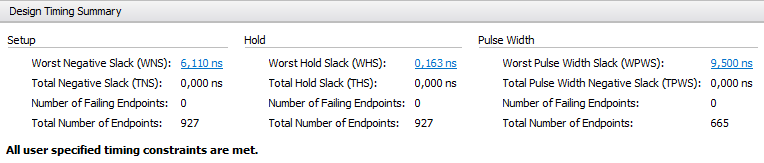
\includegraphics[width=\textwidth]{images/Vivado_timing}
\caption{Timing report from Vivado}
\label{fig:timing}
\end{figure}
% Results: power, frequency, timing, area (luts+regs)
\begin{table}[H]
    \centering
    \begin{tabular}{l|r}
        Metric & Value \\ \hline
        Power (total) & 0.133W\\
        Power (dynamic) & 0.013W \\
        Power (static) & 0.120W \\
    \end{tabular}
    \caption{Vivado power consumption}
    \label{tab:vivado_synth_results}
\end{table}
\subsection{Area utilization and performance}
The results shown in figure \ref{fig:utilization} shows the resource utilization of our design, table \ref{tab:vivado_synth_results} shows the power consumption.
\begin{figure}[H]
\centering
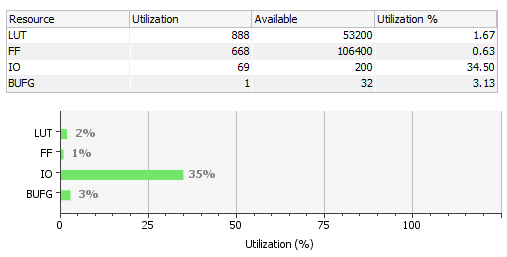
\includegraphics[width=\textwidth]{images/Vivado_utilization}
\caption{Utilization report from Vivado}
\label{fig:utilization}
\end{figure}

As the design did not pass the functionality tests there are no actual performance results available. However it is reasonable to assume that the Blakley algorithm will take 128 clock cycles to complete and the Monpro will take 129, seeing as it executes one iteration every clock cycle and there was not enough time to start optimizing the iterations by stopping earlier.\\
Therefore a rough estimate is between 
\begin{equation}
\label{equ:min_estimate}
    4+128+(128*129)+4
\end{equation} ($key_e$ of all 0's), and 
\begin{equation}
    4+128+2*(128*129)+4
\end{equation} cycles ($key_e$ of all 1's), with the average probably close to the lower of the two (\ref{equ:min_estimate}) because a small $key_e$ is common to use.


\section{Discussion of the results}
The complexity of the overall algorithm could probably have been significantly reduced if we had implemented a different algorithm for the modular exponentiation, allowing us to make more optimizations and tweak the design. \\
One thing that has been done in the Blakley module, however, is to do two different subtractions in parallell, and then choose the right result once we know what we need:

\inputminted[firstline=74,lastline=78]{VHDL}{../Project/VHDL/RSA_module.srcs/sources_1/new/blakley.vhd}

This exploits the fact that a maximum of two subtractions is necessary to make $p_{tmp} < n$ true, and actually cuts the critical path by one 128-bit adder without requiring any extra area or clock cycles. This could probably also be further optimized with regards to area, but it's probably not worth the time considering the size relative to the rest of the design.\\

\section{Further improvements}
The most obvious point to further improve on, is to actually make the state machine work correctly. Aside from that, there are multiple tricks that can be used in order to improve performance of the circuit. Both in terms of making it run at higher frequencies (by exploiting parallellism where possible) and cutting the number of required executions.\\
Probably most significant is the option to prematurely stop computing when more iterations will not make any difference, but that's a bit challenging in the algorithm that we chose.\\\\
For Monpro (see algorithm below), one possibility can be to stop once all the bits to the left of the current one are zero (in both operand a and the last intermediate result); then there will be no more additions and one only needs to right shift the result the same number of bits as there are iterations skipped. For even greater optimization, this trick could be applied even inside the computations (if there are more than one zero to the left of the current $a$ bit AND more than one zero to the right of the current result).

\inputminted[firstline=13,lastline=26]{python}{../Project/monexp.py}
